% Method overview: token-level relaxation (GReaTer) vs superposed typed blocks (GRAFT).
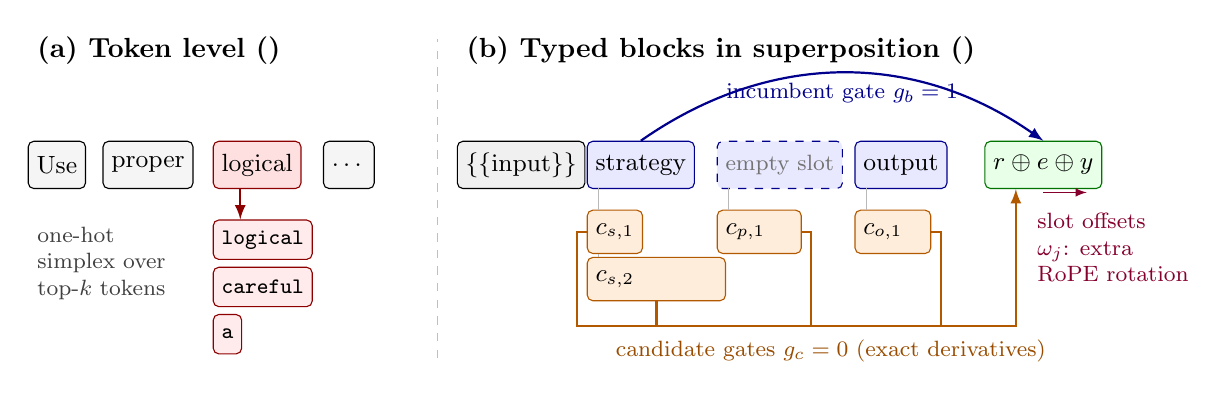
\begin{tikzpicture}[
  x=1cm, y=1cm, font=\small,
  box/.style={draw, rounded corners=2pt, minimum height=6mm, inner sep=3pt, anchor=west},
  tok/.style={box, fill=gray!8},
  alt/.style={box, fill=red!8, draw=red!55!black, minimum height=5mm, font=\footnotesize\ttfamily},
  frz/.style={box, fill=gray!12},
  inc/.style={box, fill=blue!9, draw=blue!55!black},
  cand/.style={box, fill=orange!14, draw=orange!70!black, minimum height=5.5mm},
  tail/.style={box, fill=green!9, draw=green!45!black},
  note/.style={font=\footnotesize, text=black!75, anchor=west, align=left},
  arr/.style={->, >=latex, thick},
]
% ---------------- (a) GReaTer ----------------
\node[anchor=west, font=\bfseries] at (0, 5.05) {(a) Token level (\greater{})};
\node[tok] (u) at (0, 3.6) {Use};
\node[tok] (pr) at (0.95, 3.6) {proper};
\node[tok, fill=red!12, draw=red!55!black] (lo) at (2.35, 3.6) {logical};
\node[tok] (re) at (3.75, 3.6) {\dots};
\node[alt] (a1) at (2.35, 2.65) {logical};
\node[alt] (a2) at (2.35, 2.05) {careful};
\node[alt] (a3) at (2.35, 1.45) {a};
\draw[arr, red!55!black] ([xshift=3.5mm]lo.south west) -- ([xshift=3.5mm]a1.north west);
\node[note] at (0, 2.35) {one-hot\\simplex over\\top-$k$ tokens};

\draw[gray!50, dashed] (5.2, 1.15) -- (5.2, 5.2);

% ---------------- (b) GRAFT ----------------
\node[anchor=west, font=\bfseries] at (5.45, 5.05) {(b) Typed blocks in superposition (\graft{})};
\node[frz] (x) at (5.45, 3.6) {\{\{input\}\}};
\node[inc] (s) at (7.1, 3.6) {strategy};
\node[inc, dashed, text=black!55] (p) at (8.75, 3.6) {\footnotesize empty slot};
\node[inc] (o) at (10.5, 3.6) {output};
\node[tail] (t) at (12.15, 3.6) {$r \oplus e \oplus y$};
% candidate lanes: each starts at its incumbent's first position
\node[cand] (c1) at (7.1, 2.75) {$c_{s,1}$};
\node[cand] (c2) at (7.1, 2.15) {$c_{s,2}$\,\rule{10mm}{0pt}};
\node[cand] (c3) at (8.75, 2.75) {$c_{p,1}$\,\rule{3mm}{0pt}};
\node[cand] (c4) at (10.5, 2.75) {$c_{o,1}$\,\rule{2mm}{0pt}};
\foreach \c in {c1, c3, c4} {\draw[gray!55] ([xshift=1.5mm]\c.north west) -- ++(0, 0.27);}
\draw[gray!55] ([xshift=1.5mm]c2.north west) -- ([xshift=1.5mm]c1.south west);
% incumbent gate
\draw[arr, blue!55!black] (s.north) to[out=35, in=145] node[pos=0.5, below, font=\footnotesize] {incumbent gate $g_b=1$} (t.north);
% candidate gates share a bus into the downstream tokens
\draw[orange!70!black, thick] (c1.west) -- ++(-0.12,0) |- (12.0, 1.55);
\foreach \c in {c3, c4} {\draw[orange!70!black, thick] (\c.east) -- ++(0.12,0) |- (12.0, 1.55);}
\draw[orange!70!black, thick] (c2.south) |- (12.0, 1.55);
\draw[arr, orange!70!black] (12.0, 1.55) -| ([xshift=4mm]t.south west);
\node[font=\footnotesize, text=orange!60!black, anchor=north] at (10.2, 1.5) {candidate gates $g_c=0$ (exact derivatives)};
\node[note, text=purple!70!black] at (12.7, 2.55) {slot offsets\\$\omega_j$: extra\\RoPE rotation};
\draw[->, >=latex, purple!70!black] (12.9, 3.25) -- (13.45, 3.25);
% The vertex and one-pass notes formerly drawn here are stated in the caption and in Section 3.
\end{tikzpicture}
